\chapter{Utility boards}

\section{Adapter PCB}

The adapter PCB is a small board that plugs into the controller board. Its sole purpose is to extend and route connector pins to screw terminals, allowing cables to be easily secured.

\section{Extension Terminal Socket Board}

\begin{figure}[htbp]
    \centering
    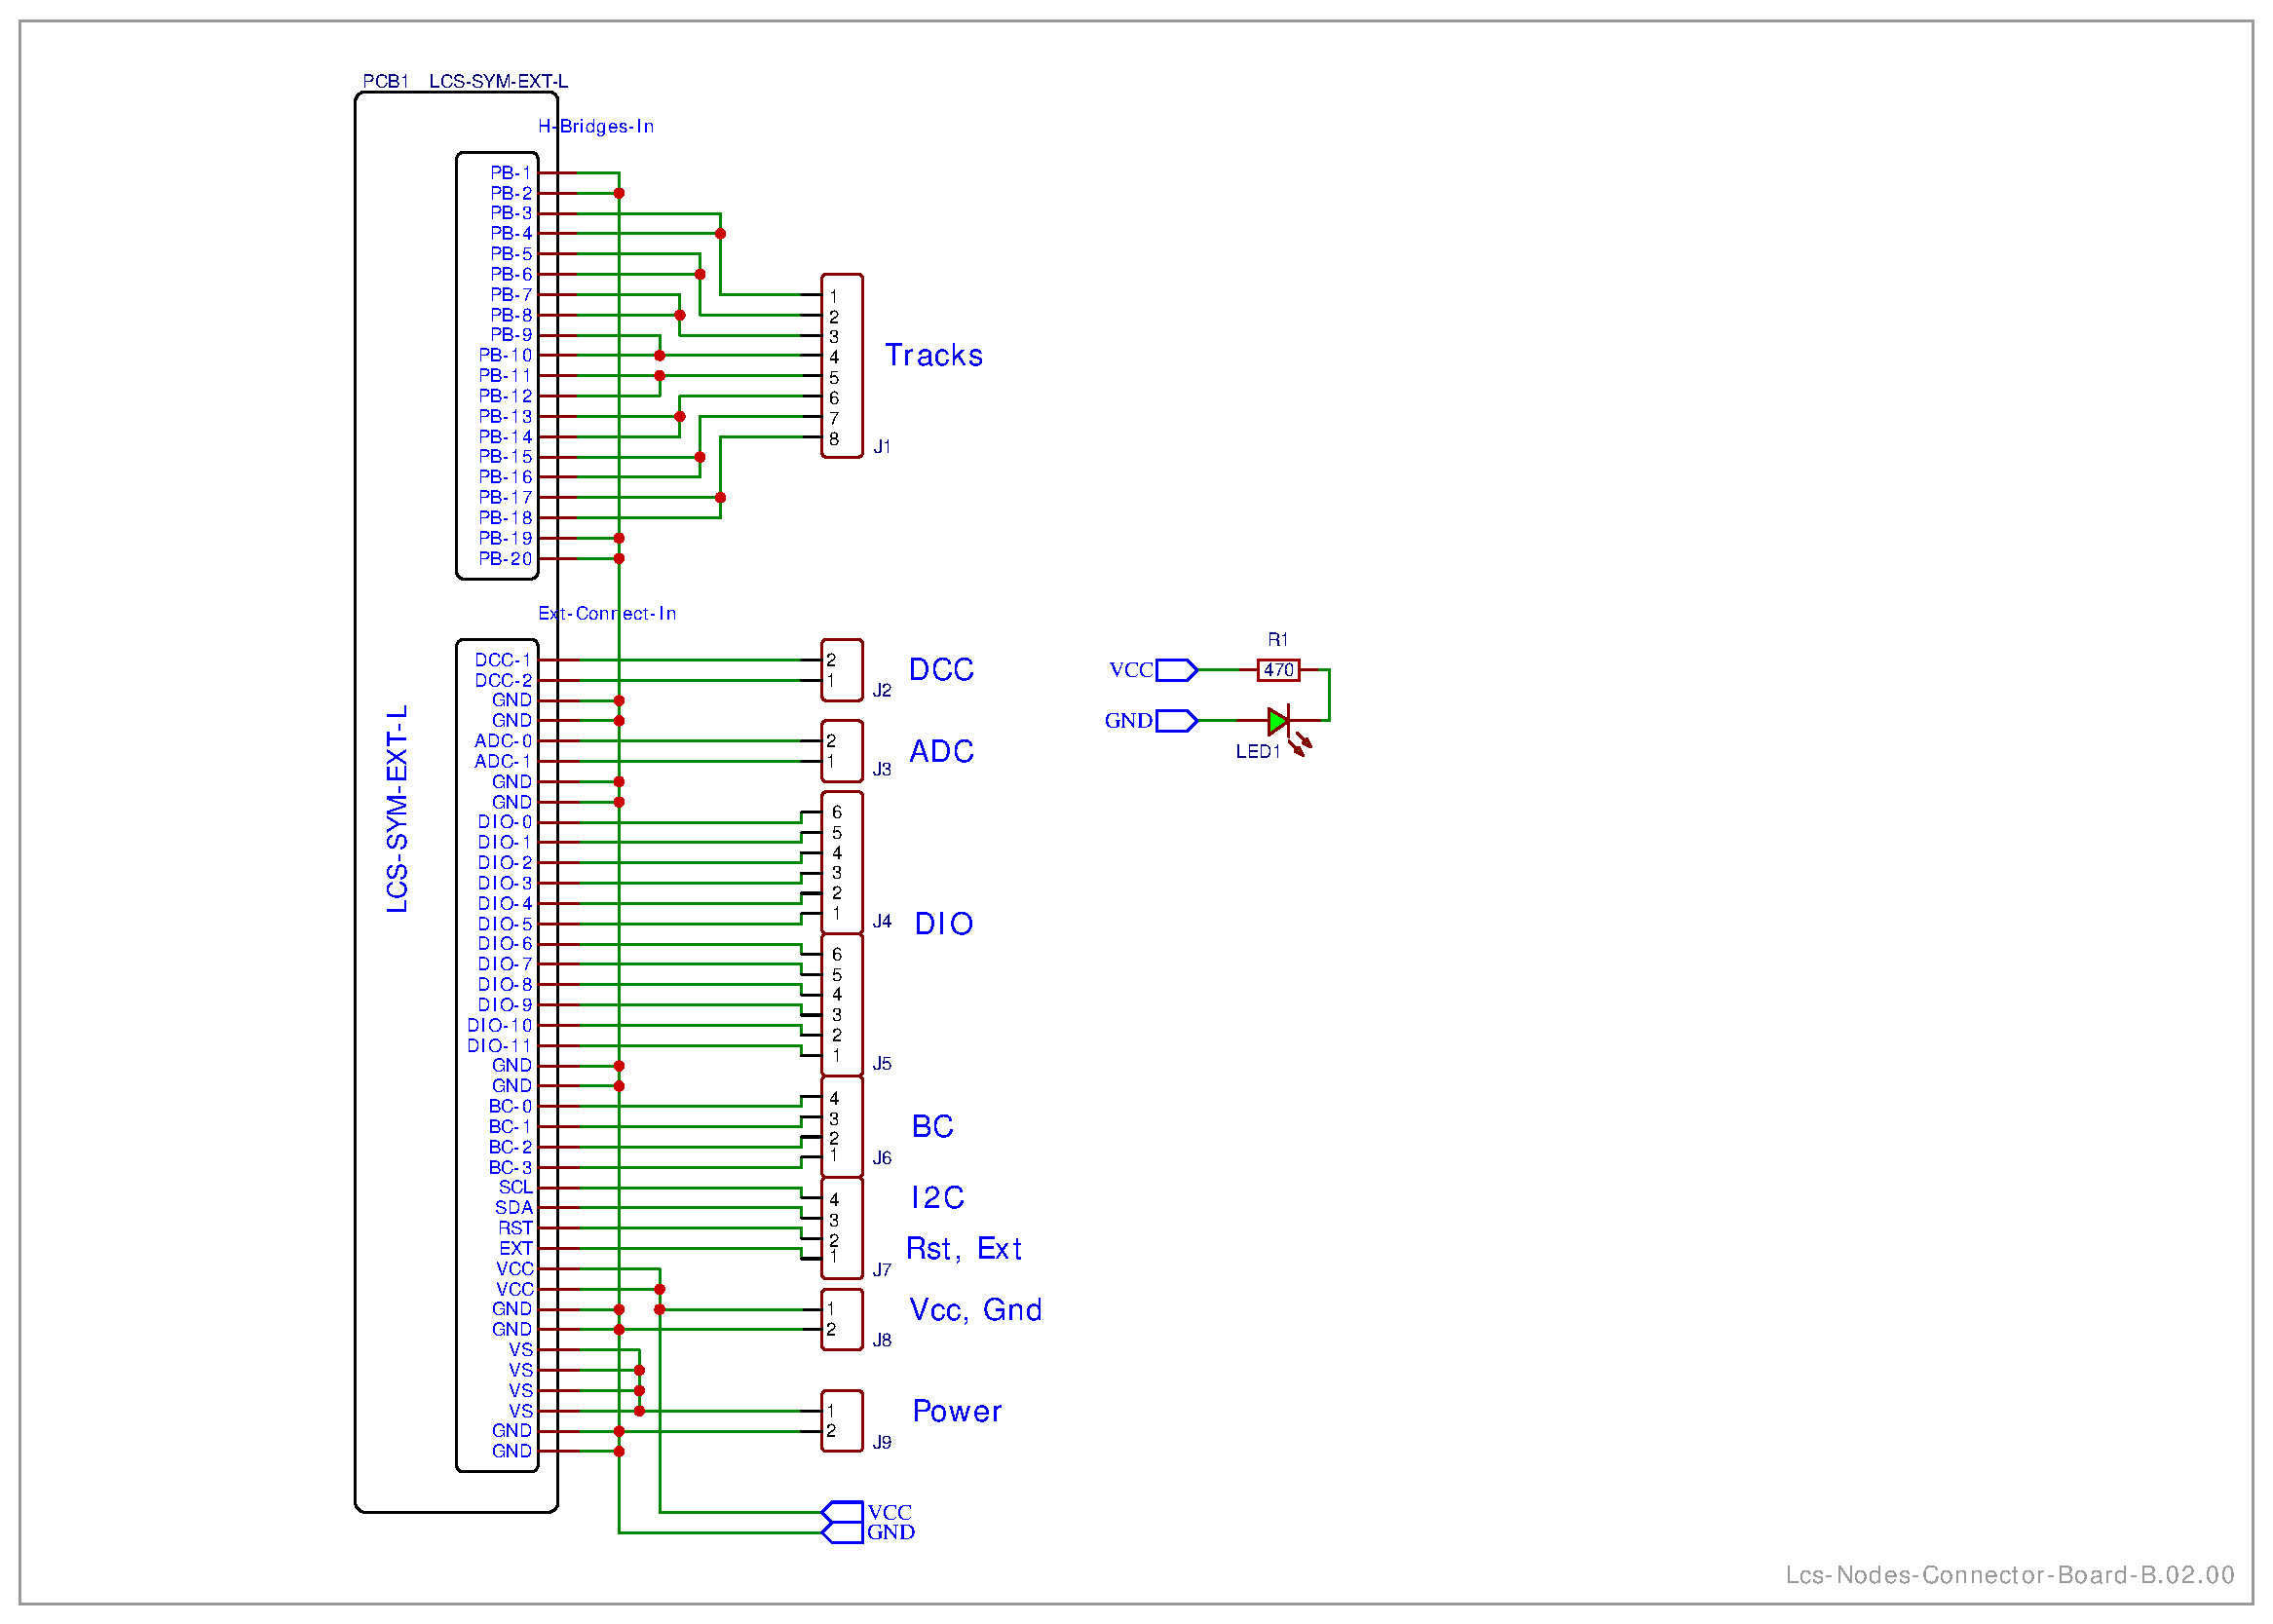
\includegraphics[page=1, width=0.9\textwidth]{./Schematics/Schematic_LcsNodes-Connector-Board.pdf}
    \caption{Block Diagram}
    %\label{fig:schematic}
\end{figure}
\FloatBarrier

\section{Extension Connector Diagnostic Board}

When developing a new controller board, testing the extension connector pins is essential. Combined with a diagnostic program, the board can be thoroughly tested. This small board plugs into the controller board to facilitate testing.

\begin{figure}[htbp]
    \centering
    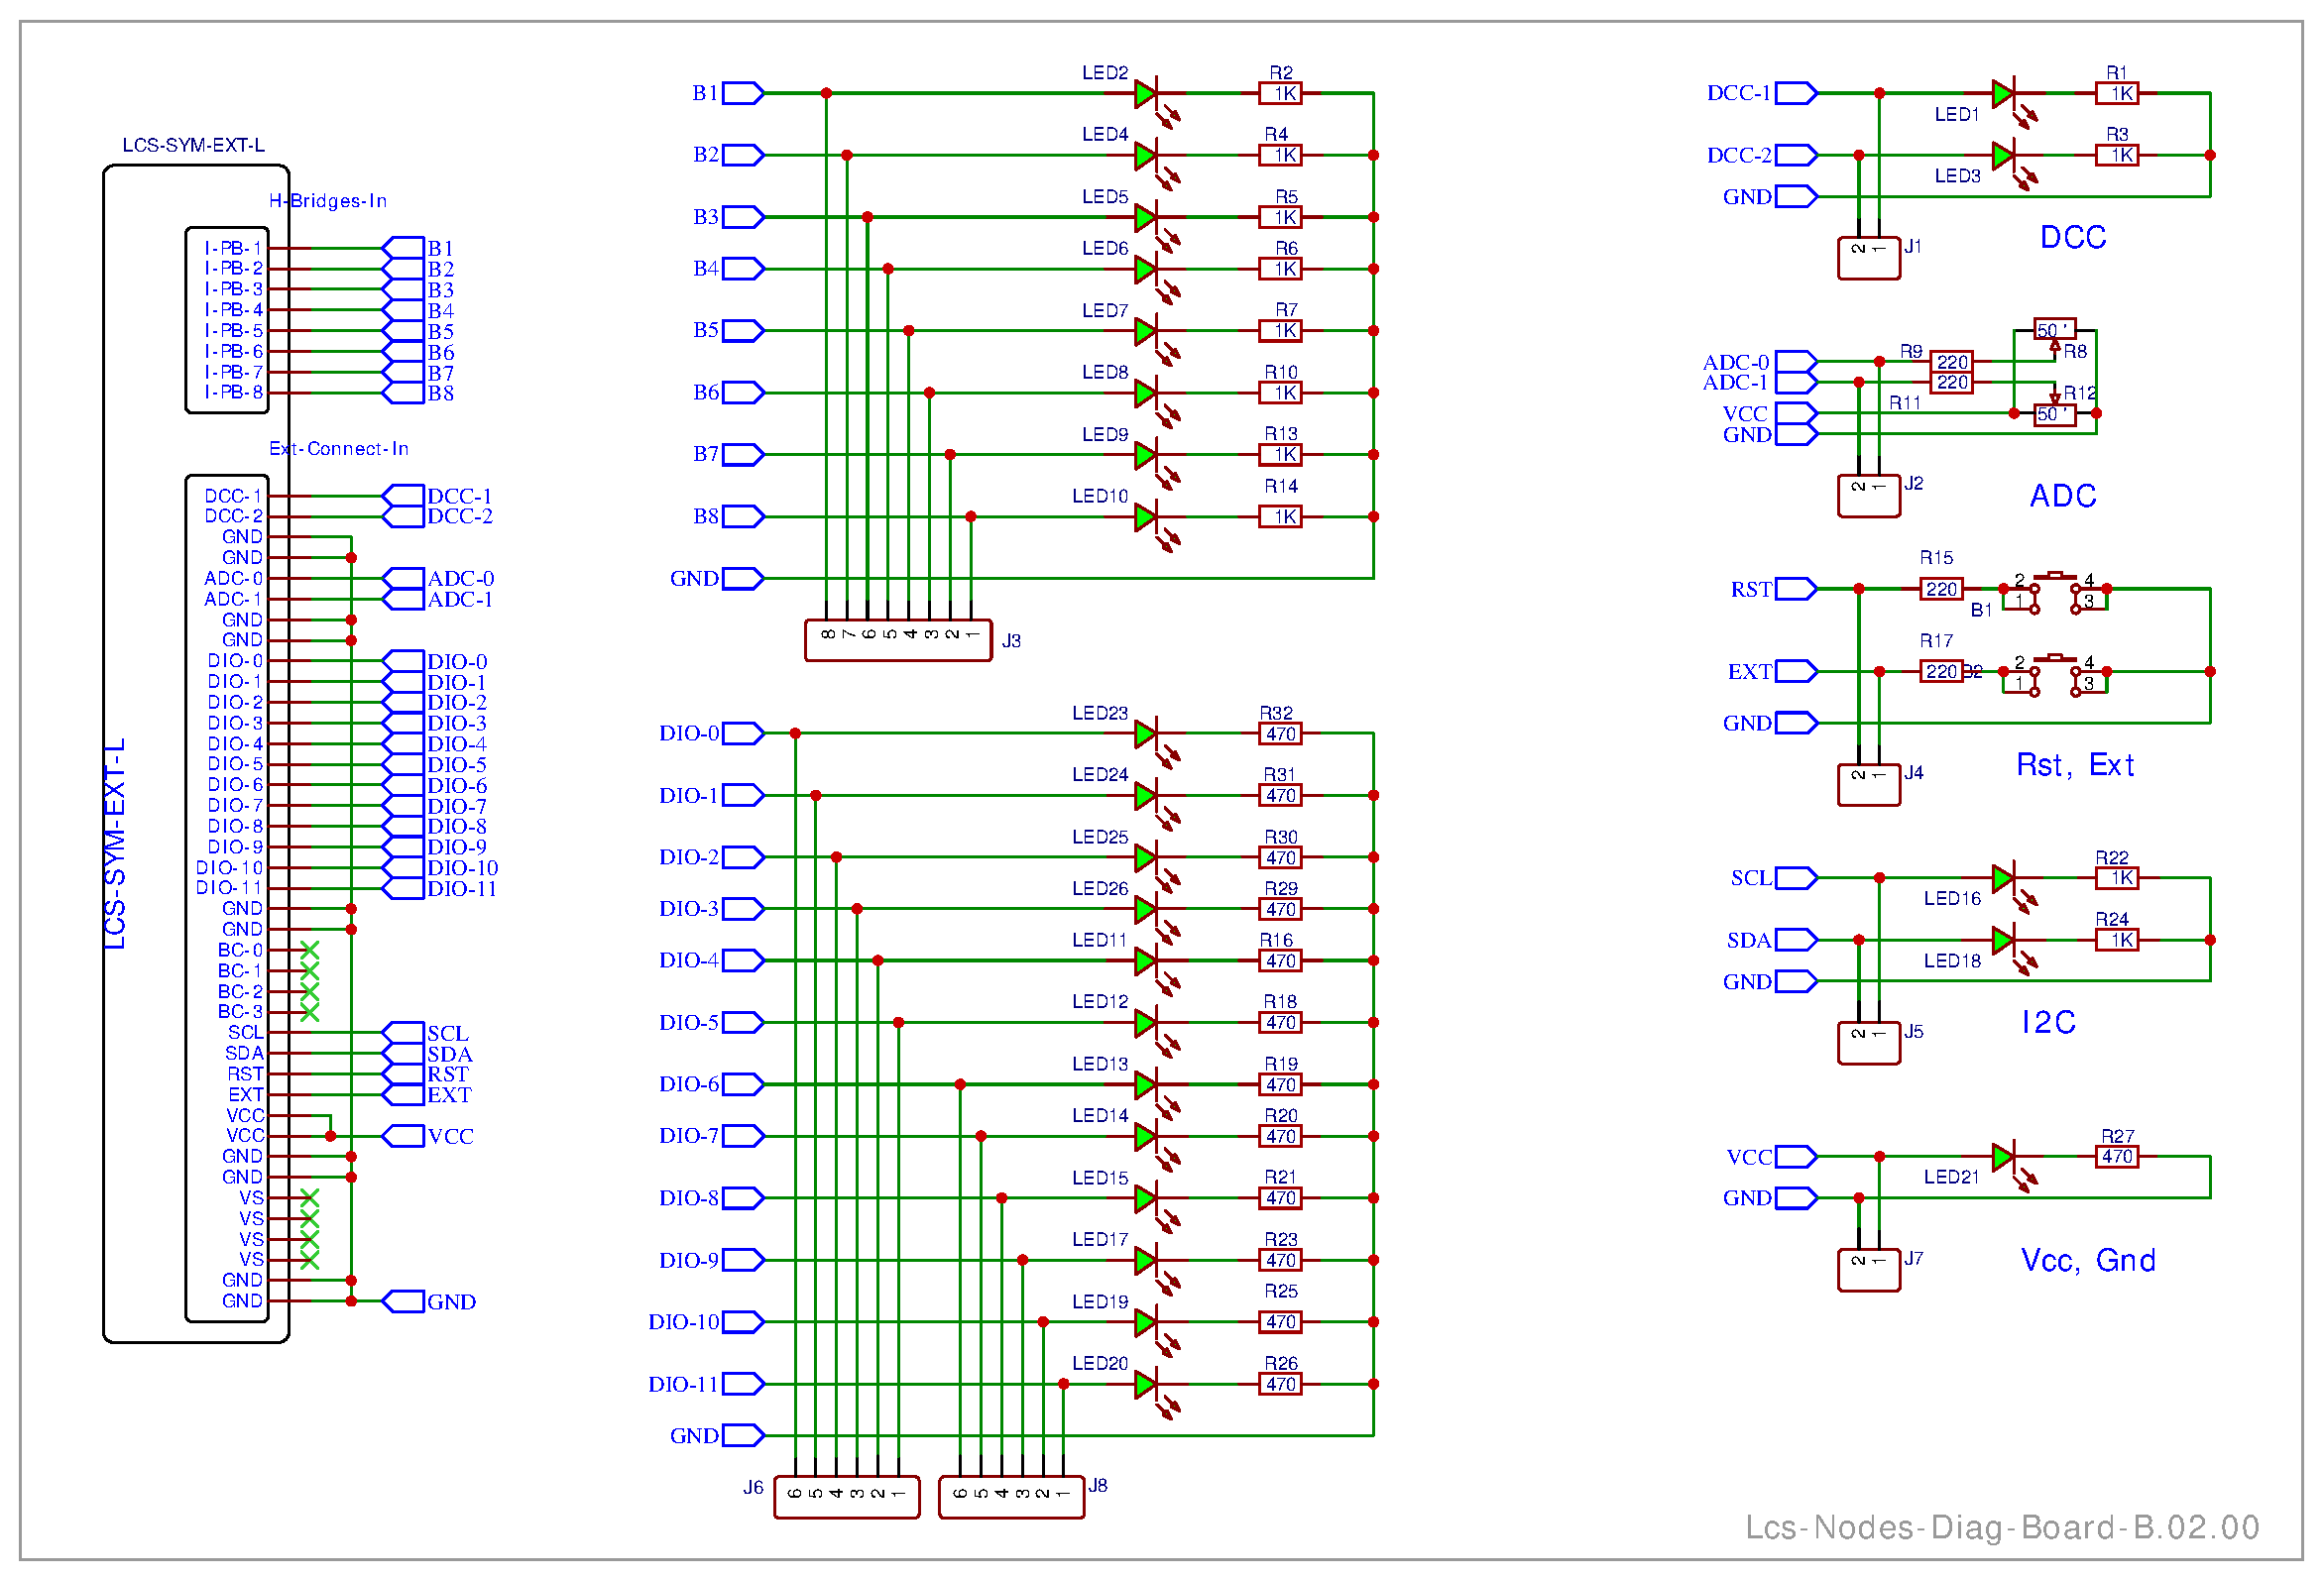
\includegraphics[page=1, width=0.9\textwidth]{./Schematics/Schematic_LcsNodes-Diagnostic-Board.pdf}
    \caption{Block Diagram}
    %\label{fig:schematic}
\end{figure}
\FloatBarrier

talk about the diagnostics. perhaps add the diagnostic program to the CDC or runtime library.

\section{BYE - Build your own extension}

Sometimes it is very useful to build a first sketch of a new extension board design. Sometimes an extension board just offers a dedicated function special to a current project and it is not worth the effort to design and build a dedicated PCB for it. In all these cases a kind of prototyping board will come in very handy. BYE is an extension board featuring NVM logic and breadboard-style rows of holes for custom designs. 

\begin{tikzpicture}[scale=0.9, transform shape]

    \draw[help lines, gray!50, dashed] (0,0) grid( 16,8);
    \node at (8,4) {picture};

\end{tikzpicture}

\subsection{Connectors and Logic}

The schematic shows the prototyping board components. All that there is, is the extension board decoding logic and the NVM for storing the configuration data. The board features all connectors, but will not route the track connectors. All in all a very simple board. Almost too simple for a block diagram.

\begin{tikzpicture}[scale=0.9, transform shape]

    \draw[help lines, gray!50, dashed] (0,0) grid( 16,8);
    \node at (8,4) {picture};

\end{tikzpicture}

\subsection{PCB}

The prototyping board is a 10cm x 12cm board with all connectors and a bread board style space for conventional components.

\begin{tikzpicture}[scale=0.9, transform shape]

    \draw[help lines, gray!50, dashed] (0,0) grid( 16,8);
    \node at (8,4) {picture};

\end{tikzpicture}

\subsection{Firmware}

Actually, there is none. Nevertheless, the board decoding logic and the local NVM memory can be used according to the prototype needs.



\section{DCC bus to digital IO}

a small board for the DCC monitoring function to derive the DCC signal...

